% Chapter 1
% !TeX spellcheck = en_US 
\chapter{Introduction} % Main chapter title

\label{Chapter1} % For referencing the chapter elsewhere, use \ref{Chapter1} 
\setcounter{chapter}{1}
%----------------------------------------------------------------------------------------

% Define some commands to keep the formatting separated from the content 
\newcommand{\keyword}[1]{\textbf{#1}}
\newcommand{\tabhead}[1]{\textbf{#1}}
\newcommand{\code}[1]{\texttt{#1}}
\newcommand{\file}[1]{\texttt{\bfseries#1}}
\newcommand{\option}[1]{\texttt{\itshape#1}}
Underlying the success of artificial intelligence are learning algorithms, i.e.,
algorithms that learn from data to perform a certain task. We start by
two concrete examples of supervised learning algorithms. In the first example we
consider the problem of approximating functions from pointwise evaluations using linear regression. In the second example we look at the task of
classifying hand-written digits. In these two examples we identify and
familiarize ourselves with the main components of learning algorithms;
\emph{datasets}, \emph{a hypothesis class}, and \emph{optimization algorithms}.
We further identify important aspects of supervised learning algorithms, such as
overfitting, and underfitting. Finally, we motivate in these two examples
problems at the forefront of research in mathematical machine learning, namely
\emph{the curse of dimensionality (CoD)} and \emph{double/multiple descent phenomenon}. 
 
\section{Supervised Learning: Motivating Examples}
In supervised learning tasks the dataset $D$ is made up of
two components, input variables $D_x = \{x_i\}_{i = 1}^N$ and targets $D_y = \{y_i\}_{i=1}^N$. The dataset is assumed to be
generated by an unknown function $f: \text{input} \to \text{target}$. The goal in
a supervised learning task is to approximate the unknown function $f$ pointwise,
i.e., to find a function $h$ such that $h(x) \approx f(x)$ for any $x$, whether
it belongs to $D_x$ or not. The target value can take finitely many values,
e.g., $\text{target} \in \{0,1, \dots, M\}$. In such a case, the supervised
learning task is called a \emph{classification task}. If the target can take
infinitely many values, the learning task is called a \emph{regression task}.  
Supervised learning problems are approached by first choosing a \emph{hypothesis
space} $\mathfrak{H}$, in which one looks for an approximation to the unknown function $f$. For example, if the data $x$ is one-dimensional and the target
take values in $\mathbb{R}$ one can define the hypothesis class to be the set of
all affine mappings, i.e., 
\begin{equation}
    \label{eq:affine_mappings}
\mathfrak{H} = \bigl\{f \ | \ f(x) = ax + b, \ a, b, \in \mathbb{R}    
\bigr\}.
\end{equation}

Then, one define a loss function $l$ that measures how well a hypothesis
function $h$ approximates an unknown function $f$ at a point $x$. Using the
dataset $D$, the supervised learning
problem can be then formulated as an optimization problem 
\begin{equation}
    \min_{h \in \frak{H}} \frac{1}{N}\sum_{i=1}^{N}l(h(x_i), y_i).
\end{equation}

While there are many alternatives to solve these optimization problems, the
by-far most used algorithms are variants of the gradient-descent algorithm. 

Let's look at some concrete examples. 

\begin{boxedexample}[Regression] \complementary{\theexample}
    \label{ex:regression}
    Let $x$ be a random variable that takes values in the interval $[-1,1]$. And assume we
    have access to a dataset $D = \{(x_i, y_i)_{i=1}^{200}\}$ generated by the unknown
    function 
    $$
    f(x) = x^2 \cos(5x) \exp(-x).
    $$ 
    Assume that the dataset is corrupted by Gaussian noise.
    To learn a function $h$ that approximates $f$ let your hypothesis class be
    the class of affine functions \eqref{eq:affine_mappings}. Let the loss
    function be the absolute error, i.e., 
    \begin{align*}
    l(h(x_i), y_i) &= |h(x_i)- y_i| \\
& = |ax_i + b - y_i|.
    \end{align*}
    Use a gradient-descent-like algorithm to choose the best hypothesis $h$,
    i.e., the best scalars $a$ and $b$. 

    Change your hypothesis class to the class of all polynomials up to   order
    20 and repeat the optimization process. Which class is better for
    optimization? \autoref{fig:regression} shows the outcome of such an experiment.
\end{boxedexample}
\begin{figure}[htbp]
    \centering
    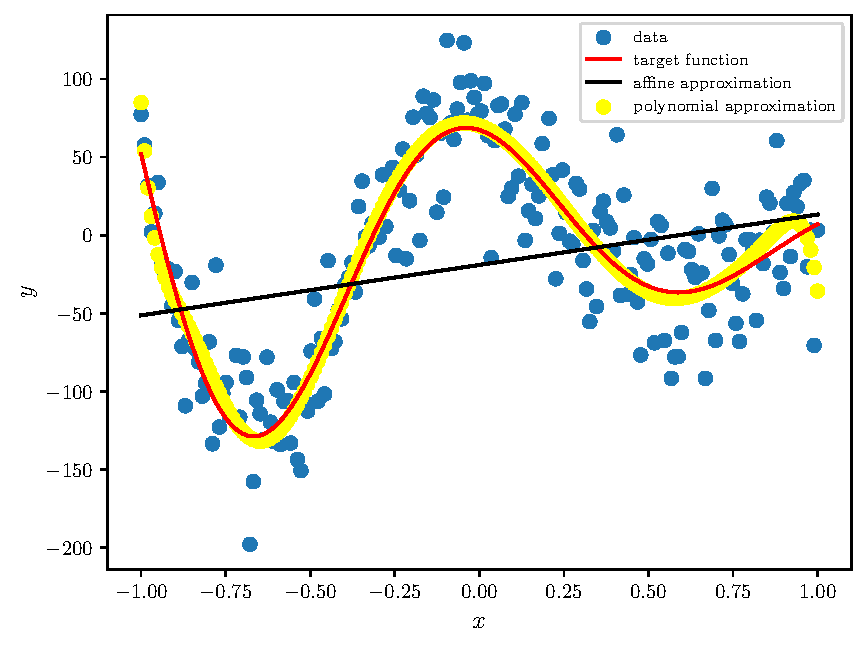
\includegraphics[width=0.8\textwidth]{Regression.pdf}
    \caption{A regression task; the goal is to fit noisy data (blue dots) assumed to be generated from a true function (solid red line). The data is fitted using an affine mapping (solid black line) and a polynomial mapping (solid yellow line).}
    \label{fig:regression}
\end{figure}   

\begin{boxedexample}[Classification] \complementary{\theexample}
    \label{ex:classification}
    We consider a classification problem of hand-written digits. The input to
    the problem is an $8 \times 8$ image of a hand-written digit, and the output
    should be the predicted value of the digit. Formally, we consider $x$ to be a
    random variable taking values in $[0, 16]^{8 \times 8} \subset
    \mathbf{N}^{8 \times 8}$, i.e., $x$ is a random variables in a matrix
    representation, where each matrix element takes an integer value between 0
    and 16. Here, the value of a certain matrix element represents its color,
    where 0 denotes black, and 16 denotes white. Let the target value $y$ be a
    random variable taking values in the discrete set $\{0,1,2,3,4,5,6,7,8,9\}$.
    To solve this supervised learning problem we consider as a hypothesis class
    the following multilayer perceptron:
    \begin{equation*}
        \mathfrak{H} = \bigl\{\text{softmax } w_2 \left(\sigma (w_1 \cdot x + b_1 ) \right) + b_2 ; w_1 \in \mathbb{R}^{\text{dh}, 8}, b_1 \in \mathbb{R}^{\text{dh}}, w_2 \in \mathbb{R}^{10, \text{dh}}, b_2 \in \mathbb{R}^{10}   \bigr\},
    \end{equation*}
    where dh is called the number of hidden units. In this class, the linear
    parameters are the weight matrices $w_1, w_2$ and the biases $b_1, b_2$.
    $\sigma$ is a nonlinear non-learnable function, often referred to by the \emph{activation function}. A common choice
    is the ReLU (Rectified Linear Unit) function
    \begin{equation*}
        \text{ReLU}(x) = \max(0, x)    
    \end{equation*}
 The softmax function (or layer) takes a set of real-valued input  and
 transforms it into a probability distribution over multiple classes. In our
 example we have ten classes and the softmax is given by
    \begin{equation*}
        \text{softmax}(z)_i = \frac{e^{z_i}}{\sum_{j=1}^{10} e^{z_j}}.
    \end{equation*}
    Therefore, the output of the hypothesis function is a probability distribution
    over the 10 classes. Concretly, the output is 10-dimensional, where each entry
    denotes the probability of the input image to represent a certain digit. 
    
    For facilitating the implementation we represent the target value as a one-hot
    vector. For example, given a target value 4, we represent it as the vector $y =
    (0,0,0,1,0,0,0,0,0,0)$. A suitable loss function for such problems is the
    categorical cross
    entropy
    function given by 
    \begin{equation*}
        l(h(x_i), y_i) = \sum_{c=0}^9 y_{i}^c \log(h(x_i)^c),
    \end{equation*}
    where $(x_i, y_i)$ is a specific training example. $y_{i}^c$ refers to the
    $c$-th entry of the one-hot vector representation of the target.

    Compute the training and test errors and study how they change when changing
    the number hidden units or number of layers.
\end{boxedexample}
  
\autoref{fig:regression} shows two hypotheses, one linear and one nonlinear, that we learned to fit the data in
\autoref{ex:regression}. The figure depicts an interesting phenomenon; a certain
hypothesis $h$ can fit the data too accurately; notice for example in
\autoref{fig:regression} that the polynomial-regression model fits badly local
minima of the target function. In these regions, it is optimized to fit the
noise. The outcome of such a result is that the polynomial-regression model will
fail to generalize well in these regions, i.e., it will have large error on
unseen data in these regions. This is called \emph{overfitting}.
On the other hand, the linear-regression model produces largely deviated from
the data everywhere, and would, hence, also generalizes badly to unseen data.
This is called an \emph{underfitting} phenomenon. 

Think about the influence of the following factor on the underfitting and
overfitting:
\begin{itemize}
    \item Complexity of the model. For a polynomial-regression model this can be
    the degree of the polynomial. 
    \item Size of the dataset. For example, would adding more data decrease or
    increase underfitting?
\end{itemize}


\section{This Course}
In this section we introduce and motivate some questions that guide the
structure of this course.  
\subsection{Generalization Error and Minimization Principles}
In \autoref{ex:classification} and \autoref{ex:regression} we saw that a model
trained on a certain dataset $D_{\text{train}}$ is expected to generalize well on \emph{unseen}
data. This is a crucial difference from standard interpolation paradigms.
Formally, the training data is assumed to follow an unknown probability
distribution $P$, i.e., $D \sim P$. It is very desirable that the learned model
not only performs well on $D$, but also on any other dataset $D_\text{test}$ that
also follows the distribution $P$. The problem is somehow ill-posed; \emph{how can one
fit a model to a training data $D$ and expect it to perform well on unseen data
$D_{\text{test}}$?}

One strategy to tackle this questions is \emph{via} induction principle.
Formally, obtaining a hypothesis that minimizes the error over the whole
distribution, also knows as the \emph{true risk}, is impossible. Instead, one
can do the next best thing. This is formally done by deriving an upper bound of
the true risk that includes, among other terms, the empirical risk, i.e., the
loss on the training data. Other terms include the so-called \emph{Rademacher
complexity}, a term which describes how complex the hypothesis class is. The
original task of minimizing the error over the whole probability distribution is
then replaced by the task of minimizing its upperbound. Such induction
strategies are called \emph{Empirical Risk Minimization Principles}. These
principles show that minimizing only the loss function of the training dataset
is not enough to obtain good generalization. One needs to regularize such loss
functions, i.e., to add some terms, whose minimization reduces the complexity of
the hypothesis class. This is directly linked to our previous discussion on
overfitting. 

The topic will be discussed in more detail in \autoref{Chapter2}.

\subsection{Hypothesis Classes and Approximation Capabilities}
In \autoref{ex:regression} and \autoref{ex:classification} we have seen some
examples of hypothesis classes, such as the class of all affine mappings, the
class of polynomials up to a predefined degree, and the class of single-layer
neural networks. Another major hypothesis class is Kernel methods. Some
important questions here are as follows: given a certain learning problem, what
class do we use? Are we guaranteed to find an optimal solution in the chosen
class? Can we increase accuracy simply by increasing the complexity of our
class?

In \autoref{Chapter3} we study two important classes of models, neural networks
and kernel methods. We survey some approximation properties of these classes and
perform error analysis for approximating important functions, such as continuous
functions, $L^p-$ functions and Sobolev functions. 

Moreover, we look with some detail at specific important application domains,
such as image recognition, and natural language processing.

\subsection{Curse of Dimensionality}
Assume that we want to optimize a potentially multi-variate unknown function $f:
\mathbb{R}^d \to \mathbb{R}$ using a dataset of
points sampled from it. Let $d=1$, i.e., assume for now that $f$ is uni-variate
and let our hypothesis class be a linear class. Denote by the $T$ the
computational costs of needed to achieve a certain accuracy $\epsilon$. It turns
out that $T$ grows exponentially with respect to $d$. In other words, the
computational costs required to achieve accuracy $\epsilon$ grow exponentially
with the dimension of the problem. This is known as the \emph{Curse of
Dimensionality} phenomenon.

Formally, when approximating an unknown function $f$ by a linear approximator
$\tilde{f}$, \emph{appriori} error estimates are often given by
\begin{equation*}
    \|f - \tilde{f}\| \leq c(d) \|f\|
\end{equation*}
where $\|.\|$ denotes some Sobolev norm of interest, and $c(d)$ is constant that
scales exponentially with the dimension of the problem. See, for example, error
bounds for approximating Schwartz functions in the linear span of Hermite
functions~\cite{Lubich:QCMD}. 
\begin{boxedexample}[CoD:Fitting] \complementary{\theexample}
    \label{ex:CoD_fitting}
Consider fitting a dataset generated from the 1-dimensional target function
\begin{equation*}
    f(x) = \cos(2x) \exp(-x),
\end{equation*}
where you use the root-mean-squared error as a loss function and a
polynomial-regression model as a hypothesis class. What is the degree of the
polynomial necessary to achieve a training set error less than $10^{-5}$.
Similarly, study the same issue for fitting a dataset generated from the 2-dimensional target function
\begin{equation*}
    f(x) = \cos(2x y) \exp(-x).
\end{equation*}
\end{boxedexample}

In fact, this phenomenon is a major bottleneck for numerical methods to solve
differential equations, such as finite differences, finite volumes or spectral
methods. 
\begin{boxedexample}[CoD:Solving Schrödinger Equation] {\theexample}
    \label{ex:CoD_TISE}
Consider the following differential operator over $\mathbb{R}^d$
\begin{equation*}
    H = -\frac{1}{2} \bigl(\Delta + |x|^2 + \frac{1}{2} |x|^4 \bigr), 
\end{equation*}
where $\Delta$ denotes the Laplacian operator, and $|x| = \sqrt{\sum_{i=1}^d |x_i|^2}$. Its eigenvalue problem reads as follows: find all eigenpairs $(E_n, \psi_n)$
that satisfy
\begin{equation*}
    H \psi_n = E_n \psi_n. 
\end{equation*}
Assume we are interested only in the smallest eigenvalue $E_0$ and its
corresponding eigenfunction $\psi_0$. Consider approximating $\psi_0$
in the linear span of truncated Hermite functions $(\gamma_n)_{n=0}^\infty$,
i.e., 
\begin{align*}
    \psi_0 &\approx \tilde{\psi}_0 \\
    &= \sum_{n=0}^{N-1} c_n \gamma_n.
\end{align*}
Set $d=1$. How many Hermite functions $N$ are necessary to approximate $E_0$ to
a relative accuracy of $10^{-1}$? Repeat the same task for $d=2$ and 3. What do you
conclude? Answers are shown in \autoref{tab:ScaleDim}. For details on
calculations refer to~\cite{Saleh:thesis:2023}.
\end{boxedexample}
\begin{table}[t]
	\centering
	\caption[Size of basis to ensure convergence for an increasing problem dimensionality]{The size of a truncated Hermite basis $N$ that is required 
	to compute the smallest eigenvalue of the differential operator in
	\autoref{ex:CoD_TISE} in
	1,2 and 3 dimensions to a relative absolute error $< 10^{-1}$.}
	\begin{tabular}{lccccc}
		\hline\hline
		$d$ &1~&2~ &3		\\
		$N$   & 3 & 45 & 286  \\
		\hline\hline
	\end{tabular}
	\label{tab:ScaleDim}
\end{table}
There is evidence, however, that neural networks are less prone to the CoD
phenomenon. In other words, the computational scaling for using them to achieve
a certain accuracy on a given task do not scale dramatically with the dimension
of the problem. Characterizing such cases and providing rigorous understanding of
this is a crucial point in modern mathematical machine learning. We will touch
on this topic in \autoref{Chapter4}. Moreover, this topic will be of major
interest to us when considering physics-informed neural networks. 

\subsection{Approximating Highly-Oscillatory Functions}
The computational costs of approximation models, whether linear or nonlinear,
seem to increase exponentially with an increase in the oscillation of a target
function. This is a major bottleneck in some applications such as quantum
dynamics. An important example here is approximating solutions to
time-independent Schrödinger equations. Similar to \autoref{ex:CoD_TISE}, the
task here is to diagonalize a differential operator that describes a certain
quantum system. We look here at a specific example, where $H$ represents an
operator, that describes vibrational motions inside a molecule. Given a linear
numerical method to compute the eigenvalues, we look in \autoref{fig:osc} at the
relative accuracy of the
first 100 eigenvalues as a function of the truncation parameter $N$. It is clear
that larger eigenvalues are harder to approximate. Morever, increasing the
truncation parameter $N$ does a worse job for improving the accuracy of higher
eigenvalues than lower eigenvalues. This is partially because, larger
eigenvalues correspond to highly-oscillatory functions. For details on the
calculations see~\cite{Saleh:arXiv2308}.

\begin{figure}[htbp]
    \centering
    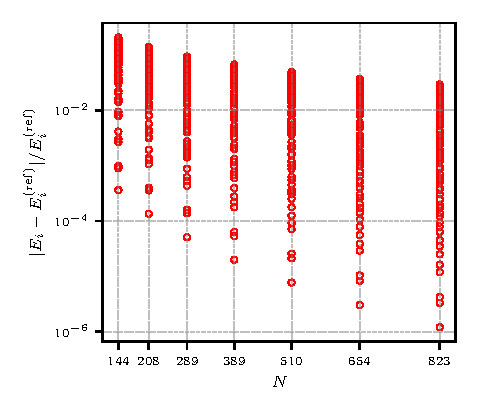
\includegraphics[width=0.8\textwidth]{H2S.pdf}
    \caption{The relative accuracy of the approximate first 100 eigenvalues of the vibrational Schrödinger equation for H$_2$S as a function of the truncation parameter $N$.}
    \label{fig:osc}
\end{figure}   
We will see in \autoref{Chapter4} that neural-network approximation methods can
significantly improve approximation capabilities for highly-oscillatory functions.
\subsection{Validity of Occam's Razor and the Overparametrized Regime}
Theoretical and empirical results have demonstrated in the past 40 years that
Occam's Razor principle is valid when dealing with machine-learning problems:
\emph{Simple solutions are favored over unnecessarily complex ones.} Indeed,
one can see in, e.g., \autoref{ex:regression} that using a very high-order
polynomial can produce very good results on the training data, but fail badly to
produce sensible predictions on unseen data, resulting in an overfitting
phenomenon. However, new evidence implies that very complex neural networks seem
to generalize well on unseen data. In particular, many of the very successul
machine-learning models that we use in our everyday life are heavily
overparamterized, i.e., they have way more optimizable parameters than training
data. Neverthess they generalize well on unseen data. Understanding the
behavior of machine-learning models in this overparameterized regime is an
important research direction in modern machine learning.

\section*{What is not covered in this course}
The field of mathematical machine learning is huge and spans many standard
mathematical areas, ranging from (geometric) measure theory to statistical
learning theory, optimization theory and functional analysis. It is hence very
challenging to cover all topics in a master course. Here is a list of topics
that we do very little to cover in this course and some references for
self-study. 

\begin{itemize}
    \item Optimizers and their convergence are largely ignored in this course.
    We use standard first order optimizers in all our numerical examples and do
    not comment on their convergence properties. 
    \item Bayesian learning models are largely marginalized.
    \item Unsupervised learning algorihtms such as clustering, and
    dimensionality reduction.
\end{itemize}

%----------------------------------------------------------------------------------------

\section*{Wait! What is what?}
Here is a list of questions that help you check your understanding of key
concepts inside this chapter.

\begin{enumerate}
    \item What are some examples of hypothesis classes? Which of them are
    linear, resp. nonlinear, approximation methods?
    \item What loss functions do you know for regression, resp. classification
    tasks? Can you think of other examples than the ones mentioned in this
    chapter?
    \item For a fitting problem, can we get more accurate results by increasing
    the complexity of the hypothesis class?
    \item How are the computational costs related to the dimension of the
    problem? 
\end{enumerate}

